
This chapter presents the governing equations for continuous and dispersed phases.

Continuous phase equations start from the compressible formulation found in \cite{poinsot2005theoretical} with the additional spray source terms. It then proceeds with the low Mach number approximation proposed in \cite{majda}. Finally, the turbulence model is presented with the extra assumptions concerning the turbulent fluxes.

Dispersed phase equations are basically those presented in \cite{nordin} and further discussed in \cite{vonkarman}, \cite{naca} and \cite{baumgarten2006mixture}.

\section{Continuous (Gaseous) Phase}

The continuous phase is the denomination for all gaseous phase in the flow
domain. The set of governing equations is composed by mass, species, momentum, energy
 and state equations. The dispersed phase will
contribute with source/sink terms for each of the gaseous phase equations and extra closure relations
will be used to account for all the phenomena complexity e.g. turbulence and
species diffusion.

All unknowns $(\rho, Y_k, \bv{U}, T)$ are functions of position and time, e.g.
$\bv{U}=\bv{U}(\bv{x},t)$. For notation reduction, however, the function
arguments will be omitted.

\subsection{Fully Compressible Formulation}

The mass (or continuity) equation for a compressible flow with the
spray source term $S_m$ is
\begin{equation}\label{ns: mass}
\frac{\partial \rho}{\partial t} + \nabla \cdot \left( \rho \bv{U} \right) =
S_m \, .
\end{equation}

\begin{remark}Since mass equation is not homogeneous due to the presence
of the spray source term, the traditional
non-conservative form of the equations must be modified. For an intensive
property $\eta$,
\begin{equation}
\begin{split}
 \frac{\partial \rho \eta}{\partial t} + \nabla \cdot \left( \rho \bv{U} \eta
\right) &= \frac{\partial \rho}{\partial t}\eta + \rho\frac{\partial
\eta}{\partial t} + \rho \bv{U} \cdot \nabla \eta + \eta \nabla \cdot \left(
\rho \bv{U} \right) \\
&= \rho \left( \frac{\partial \eta}{\partial t} + \bv{U} \cdot \nabla \eta
\right) + \eta \left[ \frac{\partial \rho}{\partial t} + \nabla \cdot \left(
\rho \bv{U} \right) \right]\\
&= \rho \left( \frac{\partial \eta}{\partial t} + \bv{U} \cdot \nabla \eta
\right) + \eta S_m \, .
\end{split}
\end{equation}
\end{remark}

Species equation with the spray source term $S_{Yk}$ is
\begin{equation}\label{ns: species}
\frac{\partial \rho Y_k }{\partial t} + \nabla \cdot \left( \rho \left( \bv{U} +
\bv{V}_{k}\right) Y_k \right) = S_{Yk} \, ,
\end{equation} where $V_k$ is the diffusion velocity of species $k$ satisfying
$\sum_{k} V_k Y_k = 0$.

The diffusion velocities will be obtained under the approximation of a dilute
mixture in which one of the species has a considerably higher concentration
relative to the others. This is the case for the spray evaporation into an air
atmosphere, where $76.7\%$ of air mass composition is nitrogen.

If $M-1$ species are present in scarce quantities relative to the last species
denoted by $M$, then these $M-1$ species diffuse as in a binary mixture:
\begin{subequations}\label{eq: byndiff}
\begin{align}
V_k Y_k &= -\mathcal{D}_k \nabla Y_k \, , \quad k=1,2,...,M-1 \, ,\\
V_M Y_M &=  \sum_{k=1}^{M-1} \mathcal{D}_k \nabla Y_k \, ,
\end{align}
\end{subequations}
where $\mathcal{D}_k$ is the binary diffusion coefficient of species $k$ and does not need
to be the same for all species.

The scarce species transport equation is then:
\begin{equation}
 \frac{\partial \rho Y_k }{\partial t} + \nabla \cdot\left( \rho Y_k \bv{U}
\right) = \nabla \cdot \left( \rho \mathcal{D}_k\nabla Y_k \right) +S_{Yk}
\, , \quad k=1,2,...,M-1.
\end{equation}


$Y_M$ is obtained from the fact that $\sum_k Y_k =1$,
\begin{equation}
Y_M = 1-\sum_{k=1}^{M-1} Y_k \, .
\end{equation}

The momentum equation is written with the assumption of a compressible Newtonian
fluid \cite{batchelor2000introduction} and includes the gravitational field
$\bv{g}$ and the spray source term $\bv{S}_{mom}$.
\begin{equation}\label{ns: momentum}
\frac{\partial \rho \bv{U} }{\partial t} + \nabla \cdot \left(\rho \bv{U}\bv{U}
\right) = -\nabla p + \nabla \cdot \bv{\tau} +\rho \bv{g}+\bv{S}_{mom} \, ,
\end{equation} where $\bv{\tau}$ is the corresponding viscous stress tensor
\begin{equation}
\bv{\tau} =  2\mu  \left[ \bv{S} -\frac{1}{3} \left( \nabla \cdot \bv{U}
\right)\bv{I} \right]\, ,
\end{equation}
and 
$\bv{S}$ is the strain tensor:
\begin{equation}
\bv{S} = \frac{1}{2} \left( \nabla\bv{U} + \nabla \bv{U}^{T} \right) \, .
\end{equation}

\begin{notation}
 $\nabla \bv{U} = \partial u_i/\partial x_j$ where $u_i$ denotes the
components of $\bv{U}$. Similarly, $\nabla \bv{U}^{T} = \partial
u_j/\partial x_i$. $\bv{I}$ denotes the identity tensor.
\end{notation}

The energy equation might be written in several different forms
(see \cite{poinsot2005theoretical}, chapter 1). Here, the sensible enthalpy
formulation will be preferred. The sensible enthalpy is defined as $h_s = h -
\sum_{k} \Delta h^{0}_{f,k} Y_k = \int_{T_{0}}^{T} c_{p} dT$, where $h$ is the
enthalpy and $\Delta h^{0}_{f,k}$ is the enthalpy of formation of species $k$ at
the reference temperature $T_{0}$.

\begin{equation}\label{ns: energy}
 \frac{\partial \rho h_s}{\partial t} +  \nabla \cdot \left( \rho h_s \bv{U}
\right) = \frac{Dp}{Dt} + \nabla \cdot \bv{J}_s +  \bv{\tau} : \nabla\bv{U} +
 S_{hs}\, ,
 \end{equation}
$S_{hs}$ is the spray enthalpy source term. $\bv{J}_s$ includes heat conduction and the enthalpy
diffusion vector:
\begin{equation}
\bv{J}_s =  \kappa \nabla T - \rho \sum_{k=1}^{M} h_{s,k} \bv{V}_k Y_k \, .
\end{equation}

With the assumptions made for species diffusion in \eqref{eq: byndiff},
$\bv{J}_s$ becomes
\begin{equation}
\bv{J}_s =  \kappa \nabla T + \rho \sum_{k=1}^{M-1} \left( h_{s,k}
-h_{s,M}\right) \mathcal{D}_k \nabla Y_k \, .
\end{equation}

\begin{notation}
 $\tau : \nabla \bv{U}$ reads in tensorial notation as following:
\begin{equation}
 \tau : \nabla \bv{U} = 2\mu\left[ \frac{1}{2} \left( \frac{\partial
u_i}{\partial x_j}+\frac{\partial u_j}{\partial x_i}\right)-\frac{1}{3}\left(
\frac{\partial u_i}{\partial x_i} \right) \delta_{ij} \right]  \frac{\partial
u_i}{\partial x_j} \, ,
\end{equation} $\delta_{ij}$ is the Kronecker delta.
\end{notation}



Constant pressure specific heat capacity for species $k$ is denoted by
$c_{p,k}$. Similarly, constant volume specific heat capacity for species
$k$ is $c_{v,k}$. The same quantities for the gaseous mixture and the
corresponding $\gamma$ constant are then
\begin{subequations}
 \begin{align}
  c_{p} &= \sum_{k} c_{p,k} Y_k \, , \\
  c_{v} &= \sum_{k} c_{p,k} Y_k \, , \\
  \gamma &= c_{p} / c_{v} \, .
 \end{align}
\end{subequations}
The gas mixture is assumed to be an ideal gas mixture and the state equation is
given by
\begin{equation}
 p =  \frac{\gamma -1}{\gamma} \rho c_p T = \frac{1}{W}\rho R T \, ,
\end{equation} where

\begin{equation}
 \frac{1}{W}=\left( \sum_k \frac{Y_k}{W_k} \right) \, .
\end{equation}





\subsection{Non-Dimensional Equations}

All equations may be written in non-dimensional form once
reference quantities are defined.
\begin{itemize}
 \item Distance is given in units of nozzle diameter $D_{jet}$;
 \item Velocity is given in units of average axial velocity
at nozzle exit $\req{U}$;
 \item Time is given in units of $ D_{jet} / \req{U}$;      
 \item Temperature is given in units of ambient temperature $T_{\infty}$;
 \item Pressure is given in units of ambient pressure $p_{\infty}$;
 \item Mass fractions are already non-dimensional;
 \item Molar mass of species k, $W_k$, is given in units of ambient air
molar mass $W_{\infty}$;
 \item Density is given in units of $\rho_{\infty}=p_{\infty} W_{\infty} / R T_{\infty}$;
 \item $c_p$ is given in units of air $c_p$ at conditions $(p_{\infty},T_{\infty})$, or
$c_{p,\infty}$. $\gamma_{\infty}$ is $c_p / c_v$ for the air at the same conditions;
 \item $h_s$ is given in units of $c_{p,\infty} T_{\infty}$.
 \item $\mathcal{D}_k$, $\mu$ and $\kappa$ are given in units of their values at ambient conditions: $\mathcal{D}_{k,\infty}$, $\mu_{\infty}$ and $\kappa_{\infty}$.
 \item $g$ is one unit of the constant gravitational field.
\end{itemize}

The following non-dimensional parameters are also defined:
\begin{subequations}
 \begin{align}
  Re &= \frac{\rho_{\infty} \req{U} D_{jet}}{\mu_{\infty}} \, ,\\
  M  &= \frac{\req{U}}{\sqrt{\gamma_{\infty} R T_{\infty}}}= \frac{\req{U}}{\sqrt{\gamma_{\infty}
  p_{\infty} /\rho_{\infty}}} \, , \\
  Pr &= \frac{\mu_{\infty} c_{p,\infty}}{\kappa_{\infty}} \, , \\
  Le_k &= \frac{\kappa_{\infty}}{\rho_{\infty} c_{p,_{\infty}} \mathcal{D}_{k,\infty}} \, , \\
  Sc_k &= \frac{\mu_{\infty}}{\rho_{\infty} \mathcal{D}_{k,\infty}} = Pr Le_k \, , \\
  Fr &= \frac{\req{U}}{\sqrt{g D_{jet}}} \, .
 \end{align}
\end{subequations}

Equations are then rewritten in terms of non-dimensional quantities.
\begin{description}
\item[State equation:]
\begin{equation}\label{nd: state}
p=\rho T \left( \sum_k \frac{Y_k}{W_k}\right) = \frac{\rho T}{W} \, .
\end{equation}
\item[Mass equation:]
\begin{equation}\label{nd: mass}
\frac{\partial \rho}{\partial t} + \nabla \cdot \left( \rho \bv{U} \right) = 
S_m \, .
\end{equation}
\item[Species equation:]
\begin{subequations}\label{nd: species}
\begin{equation}
 \frac{\partial \rho Y_k }{\partial t} + \nabla \cdot\left(\rho \bv{U} Y_k
\right) = \frac{1}{Re Sc_k} \nabla \cdot \left( \rho \mathcal{D}_k \nabla Y_k
\right) +S_{Yk} \, , \quad k=1,2,...,M-1 \, .
\end{equation}
\begin{equation}
Y_M = 1- \sum_{k=1}^{M-1} Y_k \, .
\end{equation}
\end{subequations}
\item[Momentum equation:]
\begin{equation}\label{nd: momentum}
 \frac{\partial \rho \bv{U} }{\partial t} + \nabla \cdot \left( \rho \bv{U}
\bv{U} \right) = -\frac{1}{\gamma_{\infty} M^2} \nabla p + \frac{1}{Re} \nabla \cdot
\bv{\tau} +\frac{\rho}{Fr^2} \frac{\bv{g}}{|\bv{g}|}+\bv{S}_{mom} \, .
\end{equation} 
\item[Energy equation:]
\begin{equation}\label{nd: enthalpy}
\begin{split}
\frac{\partial \rho h_s}{\partial t} +  \nabla \cdot \left(\rho \bv{U} h_s
\right) &= \frac{\gamma_{\infty} -1}{\gamma_{\infty}}\frac{Dp}{Dt} + \nabla \cdot \bv{J}_s \\
&+ M^2 \left( \gamma_{\infty}-1 \right) \left( \frac{\bv{\tau} : \nabla\bv{U}}{Re}  \right) + S_{hs}\, ,
\end{split}
\end{equation} 
\end{description}

where $\bv{\tau}$ is the shear stress tensor \begin{equation}
\bv{\tau} =  2 \mu \left[ \bv{S} -\frac{1}{3} \left( \nabla \cdot \bv{U}
\right)\bv{I} \right]\, ,
\end{equation}
$\bv{I}$ is the identity tensor and $\bv{S}$ is the strain tensor
\begin{equation}
\bv{S} = \frac{1}{2} \left( \nabla\bv{U} + \nabla \bv{U}^{T} \right) \, .
\end{equation}
$\bv{J}_s$ is the heat conduction and the sensible enthalpy diffusion:
\begin{equation}
\bv{J}_s =  \frac{\kappa}{Re Pr} \nabla T + \sum_{k=1}^{M-1} \frac{\rho
\mathcal{D}_k}{Re Sc_k} \left( h_{s,k} -h_{s,M} \right) \nabla Y_k  \, .
\end{equation}

\subsection{Low Mach Number Approximation}
Consider the following definitions \cite{viozat1997implicit}:

\begin{quote}
A \textbf{compressible flow} is a flow in which density depends on pressure and
temperature.
\end{quote}

\begin{quote}
A \textbf{dilatable flow} is a flow in which density depends on temperature.
\end{quote}

The gas flow considered in this work is fairly incompressible, indeed the
local Mach number is below $0.1$ throughout the flow domain. However, the
intense heat and mass transfers between gaseous and liquid phases when
spray is present produce large temperature gradients which cause density to vary
considerably and the two-phase flow may be classified as a dilatable flow in the
sense of the definition above.

An important difference between incompressible and dilatable flows is
that $\nabla \cdot \bv{U} = 0$ does not hold for the latter. 

A common treatment for dilatable flows is the low Mach number approximation, which consists in expanding unknown quantities $p$, $Y_k$, $\bv{U}$ and $T$ in Equations \eqref{ns:
mass}, \eqref{ns: momentum} and \eqref{ns: energy} into power series
of $\xi \equiv \sqrt{\gamma_{\infty}} M$:
\begin{subequations}\label{eq: expansion}
 \begin{align}
   p &= p_{0} + p_{1}\xi + p_{2}\xi^2 + O\left( \xi^3 \right) \, ,\\
   Y_k &= Y_{k,0} + O\left( \xi \right) \, ,\\
  \bv{U} &= \bv{U}_{0} + O\left( \xi \right) \, ,\\
  T &= T_{0} + O\left( \xi \right) \, .
 \end{align}
\end{subequations}

The reason for expanding pressure up to the second order while keeping only the
leading (or zeroth) order for the other variables is discussed in
\cite{muller1999low}, but it is essentially because of the $M^{-2}$ factor in momentum equation \eqref{nd: momentum}. 

The dependence of the spray source terms on the flow variables is also considered only for the leading order.

$\rho_0$ is obtained by substitution of \eqref{eq: expansion} into the
non-dimensional state equation. $\rho_0$ is such that
\begin{equation}\label{lm: state}
 p_0 = \rho_0 T_0 \left( \sum_k \frac{Y_{k,0}}{W_k} \right) =  \frac{ \rho_0
T_0}{W_0}\, .
\end{equation}

Mass equation \eqref{nd: mass} of order $\xi^0$ becomes:
\begin{equation}
 \frac{\partial \rho_0}{\partial t} + \nabla \cdot \left( \rho_0 \bv{U}_0
\right) =  S_m \, .
\end{equation}

Species equation \eqref{nd: species} of order $\xi^0$ is:
\begin{subequations}\label{lm: species}
\begin{align}
 \frac{\partial \rho_0 Y_{k,0} }{\partial t} + \nabla \cdot\left(\rho_0 \bv{U}_0
Y_{k,0} \right) &= \frac{1}{Re Sc_k} \nabla \cdot \left( \rho \mathcal{D}_k
\nabla Y_{k,0} \right) +S_{Yk} \, , \quad k=1,2,...,M-1 \, . \\
  Y_{M,0} &= 1- \sum_{k=1}^{M-1} Y_{k,0} \, .
\end{align}
\end{subequations}

The momentum equation gives information of orders $\xi^{-2}$, $\xi^{-1}$ and
$\xi^0$ due to the presence of the coefficient $1/\xi^2$ in the pressure gradient . The
resulting equations are, respectively,
\begin{subequations}\label{lm: momentum}
\begin{align}
 \nabla p_0 &\equiv 0 \, , \\
 \nabla p_1 &\equiv 0 \, , \\
 \frac{\partial \rho_0 \bv{U}_0 }{\partial t} + \nabla \cdot \left( \rho_0
\bv{U}_0 \bv{U}_0 \right) &= -\nabla p_2 + \frac{1}{Re} \nabla \cdot \bv{\tau}_0
+\frac{\rho_0}{Fr^2} \frac{\bv{g}}{|\bv{g}|}+\bv{S}_{mom}  \, .
\end{align}
\end{subequations}

From $\nabla p_0 \equiv \nabla p_1 \equiv 0$, it is observed that $p_0$ and
$p_1$ are functions of time only, $p_0 = p_0 (t)$ and $p_1 = p_1 (t)$. The
coupling between  velocity and pressure fields is now separated into two
contributions:  $p_2$ establishes the pressure gradient and will be referred to
as the dynamic pressure; $p_0$ affects $\rho_0$ via the state equation and will
be referred to as the thermodynamic pressure. 

The energy equation reads
\begin{equation}\label{lm: enthalpy}
\frac{\partial \rho_0 h_{s0}}{\partial t} +  \nabla \cdot \left(\rho_0 \bv{U}_0
h_{s0} \right) = \frac{\gamma_{\infty} -1}{\gamma_{\infty}}\frac{Dp_0}{Dt} + \nabla \cdot
\bv{J}_{s0} + S_{hs}\, ,
\end{equation} where 
\begin{equation}
\bv{J}_{s0} =  \frac{\kappa}{Re Pr} \nabla T_0 + \sum_{k=1}^{M-1}
\frac{\rho\mathcal{D}_k}{Re Sc_k} \left( h_{s0,k} -h_{s0,M} \right) \nabla
Y_{k,0} \, . 
\end{equation}

An ordinary differential equation in time may be derived for computing the thermodynamic pressure ($p_0$) by differentiating the state equation \eqref{lm: state} with respect to time and integrating in domain volume:
\begin{equation}\label{lm: dstate}
 \frac{Dp_0}{Dt}\int_{\Omega}W dV + p_0 \int_{\Omega}\frac{DW}{Dt} dV=\int_{\Omega} \frac{D\rho T}{Dt} dV\, ,
\end{equation}
where 
\begin{equation}
\frac{D}{Dt} = \frac{\partial}{\partial t}+\bv{U}\cdot\nabla
\end{equation}
is the total derivative.

Each total derivative may be computed from mixture molar mass ($W$) definition and mass, species and enthalpy equations. 

For an infinite (or open) domain $\Omega$, 
\begin{equation}
\int_{\Omega}\frac{DW}{Dt} dV < \infty \, , \quad \int_{\Omega} \frac{D\rho T}{Dt} dV < \infty \quad \text{and} \quad \int_{\Omega}W dV = \infty \, .
\end{equation}
 Hence, $Dp_0/Dt = 0$ and $p_0 = 1$, the non-dimensional pressure in far-field boundary.

Herein, the subscripts denoting the order of expansion will be omitted, except
for the pressure. $\bv{U}_0$ is simply $\bv{U}$ and the same holds to $\rho$,
$Y_k$, $h_s$ and $T$. For pressure, $p_0$ is the thermodynamic pressure and
$p_2$ is the dynamic pressure.

\subsection{Turbulence Modeling}

The expression \textit{turbulent and evaporating spray} entitling this work
refers to a liquid spray evolving in a gaseous turbulent flow where mass, energy
and momentum transfers between both phases are strongly affected by turbulence. 

Among all possible treatments for turbulent flows, see
\cite{pope2000turbulent}, one is perhaps the most widely used in industrial
applications: the so called \textit{standard k-epsilon model}. This two-equation
model within the RANS (Reynolds-averaged Navier-Stokes) framework provides a good
compromise between complexity and computational cost for those not using
exceptional computational resources. 

In the context of RANS modeling, the governing equations are averaged and solved
for the mean values of flow properties. The effect of turbulence on the mean
field is accounted by modeling the terms depending on the fluctuations. In the
specific case of the momentum equation, the hypothesis of turbulent-viscosity
(or Boussinesq hypothesis) is used to compute an effective value of local
viscosity composed by molecular and turbulent viscosities, being the
latter an approximation of the extra momentum flux of Reynolds stresses.

For compressible flows, two averages are commonly used: the simple time average
and a mass-weighted time average (or Favre average), see \cite{favre1969statistical}.
The time average $(\bar{f})$ and the deviation $(f')$  of a quantity $f$ are
defined as
\begin{equation}
 \bar{f}(x,t) \equiv \frac{1}{T}\int_{t}^{t+T} f(x,\tau) d\tau \quad \text{and}
\quad f'(x,t)= f(x,t)-\bar{f}(x,t) \, .
\end{equation}

The mass-weighted average (or Favre average) $(\tilde{f})$ and the deviation
$(f'')$ are defined as
\begin{equation}
 \tilde{f}(x,t) = \frac{\overline{\rho f(x,t)}}{\bar{\rho}} \quad \text{and}
\quad f^{''}(x,t) = f(x,t) - \tilde{f}(x,t) \, .
\end{equation}

Following the definitions,
\begin{equation}
 \quad \overline{f'}=\bar{f}-\bar{f}=0 \quad \text{and} \quad \bar{\bar{f}}=
\bar{f}\, ,
\end{equation}
\begin{equation}
 \quad \tilde{f''}=\tilde{f}-\tilde{f}=0 \quad \text{and} \quad \tilde{\tilde{f}}=
\tilde{f}\, .
\end{equation}
Averaging and differential operators are assumed to commute, see \cite{pope2000turbulent}. 

\subsubsection{Mass and Species Equations}
Averaged mass and species equations are easily obtained. The
averaged mass equation reads:
\begin{equation}\label{av: mass}
  \frac{\partial \bar{\rho}}{\partial t} + \nabla \cdot \left( \bar{\rho}
\tilde{\bv{U}} \right) =  \bar{S}_m \, .
\end{equation}

The species averaged equation reads:
\begin{subequations}\label{av: species1}
\begin{equation}
 \frac{\partial \bar{\rho} \tilde{Y}_k }{\partial t} + \nabla
\cdot\left(\bar{\rho} \tilde{\bv{U}} \tilde{Y}_k +\bar{\rho}\widetilde{\bv{U''}
Y''_{k}} \right) = \frac{1}{Re Sc_k} \nabla \cdot \left( \overline{\rho
\mathcal{D}_k \nabla Y_k} \right) +\bar{S}_{Yk} \, , \quad k=1,2,...,M-1 \, ,
\end{equation}
\begin{equation}
\tilde{Y}_M = 1- \sum_{k=1}^{M-1} \tilde{Y}_{k} \, .
\end{equation}
\end{subequations}
Equation \eqref{av: species1} shows two new terms: $\overline{\rho \mathcal{D}_k \nabla
Y_k}$ and $\bar{\rho}  \widetilde{\bv{U}'' Y_k^{''}}$. Unless new equations are
derived for them, both terms are not known and must be modeled.

For the first one, regarding the laminar diffusivity of species, the average is
commonly approximated as shown below:
\begin{equation}
\overline{\rho \mathcal{D}_k \nabla Y_k} \approx \bar{\rho}\mathcal{D}_k \nabla
\tilde{Y}_k \, .
\end{equation}

For the second term, which deals with turbulent flux, an approach analogous
to turbulent-viscosity is used and a turbulent coefficient for species
diffusion $(\mathcal{D}_{k,t})$ is used:
\begin{equation}
\bar{\rho}  \widetilde{\bv{U}'' Y_k^{''}} \approx -\frac{\bar{\rho}
\mathcal{D}_{k,t}}{Re Sc_k} \nabla \tilde{Y}_k \, ,
\end{equation}
$\mathcal{D}_{k,t}$ is computed by the turbulence model.

The species equation then becomes:
\begin{subequations}\label{av: species}
\begin{equation}
 \frac{\partial \bar{\rho} \tilde{Y}_k }{\partial t} + \nabla
\cdot\left(\bar{\rho} \tilde{\bv{U}} \tilde{Y}_k \right) = \frac{1}{Re Sc_k}
\nabla \cdot \left[ \bar{\rho} \left( \mathcal{D}_k + \mathcal{D}_{k,t} \right)
\nabla \tilde{Y}_k \right] +\bar{S}_{Yk} \, , \quad k=1,2,...,M-1 \, .
\end{equation}
\begin{equation}
\tilde{Y}_M = 1- \sum_{k=1}^{M-1} \tilde{Y}_{k} \, .
\end{equation}
\end{subequations}

\subsubsection{Momentum Equation}
Treatment of momentum equation is more complicated and it is shown in more
steps here. The averaged momentum equation reads:
\begin{equation}
 \frac{\partial \bar{\rho} \tilde{\bv{U}} }{\partial t} + \nabla \cdot \left(
\bar{\rho} \tilde{\bv{U}} \tilde{\bv{U}} \right) = -\nabla \bar{p}_2 +  \nabla
\cdot \left(  \frac{\bar{\bv{\tau}}}{Re} - \bar{\rho}\widetilde{\bv{U}''
\bv{U}''} \right) +\frac{\bar{\rho}}{Fr^2}
\frac{\bv{g}}{|\bv{g}|}+\bar{\bv{S}}_{mom}  \, .
\end{equation}

Again, two terms are new and unknown: $\bar{\tau}$ and $-
\bar{\rho}\widetilde{\bv{U}'' \bv{U}''}$. From the definitions of averages, 
\begin{equation}
 \tau = \tilde{\tau}+\tau'' \quad \Rightarrow \quad \bar{\tau} =
\tilde{\tau}+\overline{\tau''} \, ,
\end{equation}
and assuming $\tilde{\tau} \gg \overline{\tau''}$, we have:
\begin{equation}
 \bar{\tau} \approx  2\mu\left[ \tilde{S}-\frac{I}{3}\left(\nabla \cdot
\tilde{\bv{U}} \right)  \right] \, .
\end{equation}

The modeling of the turbulent momentum flux is made by the following
expression (known as Boussinesq hypothesis):
\begin{equation}\label{eq: boussinesq}
 - \bar{\rho}\widetilde{\bv{U}'' \bv{U}''} =  \frac{2 \mu_t}{Re} \left[
\tilde{S}-\frac{I}{3} \left( \nabla \cdot \tilde{\bv{U}} \right)  \right] -
\frac{2}{3}\bar{\rho}kI \, .
\end{equation}

$\mu_t$ is the turbulent-viscosity accounting for the extra momentum flux due to the Reynolds stresses ($-
\bar{\rho}\widetilde{\bv{U}'' \bv{U}''}$). $k$ is turbulent kinetic energy defined as:
\begin{equation}
  k = \frac{1}{2} \widetilde{\left(\bv{U}'' \cdot \bv{U}'' \right) \, .}
\end{equation}
Both $\mu_t$ and $k$ are computed by the turbulence model.

$\tau_{tot}$ is defined as a ``new viscous stress tensor'' composed by the
laminar and turbulent part:
\begin{equation}
 \overline{\tau_{tot}} \equiv 2 (\mu + \mu_t) \left[
\tilde{S}-\frac{I}{3}\left(\nabla \cdot \tilde{\bv{U}} \right)  \right]
-\frac{2}{3}\bar{\rho}k I \, ,
\end{equation}
and the momentum equation finally becomes:
\begin{equation}\label{av: momentum}
 \frac{\partial \bar{\rho} \tilde{\bv{U}} }{\partial t} + \nabla \cdot \left(
\bar{\rho} \tilde{\bv{U}} \tilde{\bv{U}} \right) = -\nabla \bar{p}_2 +  
\frac{1}{Re}  \nabla \cdot\overline{\bv{\tau}_{tot}} +\frac{\bar{\rho}}{Fr^2}
\frac{\bv{g}}{|\bv{g}|}+\bar{\bv{S}}_{mom}  \, .
\end{equation}

\subsubsection{Sensible Enthalpy Equation}
The averaged sensible enthalpy equation reads:
\begin{equation}
\frac{\partial \bar{\rho} \tilde{h}_{s}}{\partial t} + \nabla \cdot
\left(\bar{\rho} \tilde{\bv{U}} \tilde{h}_{s} + \bar{\rho} \widetilde{\bv{U}''
h_s^{''}} \right) = \frac{\gamma_{\infty} -1}{\gamma_{\infty}}\overline{\frac{Dp_0}{Dt}} + \nabla
\cdot \bar{\bv{J}}_s + \bar{S}_{hs}\, ,
\end{equation} where 
\begin{equation}
\bv{J}_s =  \overline{\frac{\kappa}{Re Pr} \nabla T} + \sum_{k=1}^{M-1}
\overline{\frac{\rho\mathcal{D}_k}{Re Sc_k} \left( h_{s,k} -h_{s,M} \right)
\nabla Y_{k}} \, . 
\end{equation}

Four new terms are unknown and must be modeled as well:\\  $\bar{\rho}
\widetilde{\bv{U}'' h_s^{''}} $ , $\overline{\frac{Dp}{Dt}} $, 
$\overline{\frac{\kappa}{Re Pr} \nabla T}$ and 
$\overline{\frac{\rho\mathcal{D}_k}{Re Sc_k} \left( h_{s,k} -h_{s,M} \right)
\nabla Y_{k}} $.

Turbulent flux of enthalpy is modeled similarly to species and momentum
turbulent fluxes:
\begin{equation}
 \bar{\rho} \widetilde{\bv{U}'' h_s^{''}} \approx -\frac{\bar{\rho} \alpha_t
}{Re Pr} \nabla \tilde{h}_s \, ,
\end{equation}
where $\alpha_t$ is the turbulent thermal diffusivity that is also computed by the
turbulence model.

The average of the total derivative $\overline{Dp/Dt}$ reads:
\begin{equation}
 \overline{\frac{D p_0}{D t}} = \frac{\partial \bar{p}_0}{\partial
t}+\overline{\bv{U} \cdot \nabla p_0} = \frac{\partial \bar{p}_0}{\partial t} + \left( \tilde{\bv{U}} \cdot \nabla \bar{p}_0 \right) + \overline{\bv{U}'' \cdot \nabla p_0}
\end{equation}
Neglecting the last term ($\overline{\bv{U}'' \cdot \nabla p_0}$) gives:
\begin{equation}
 \overline{\frac{D p_0}{D t}}  \approx \frac{\partial \bar{p}_0}{\partial t} +
\left( \tilde{\bv{U}} \cdot \nabla \bar{p}_0 \right)\, .
\end{equation}

For laminar heat diffusion, the effect of fluctuations is neglected and only
averaged terms are considered:
\begin{equation}
 \overline{k \nabla T} = \bar{k} \nabla \tilde{T} + \overline{k\nabla T''}
\approx \bar{k} \nabla \tilde{T} \, .
\end{equation} 

Under the same assumption:
\begin{equation}
 \overline{\frac{\rho \mathcal{D}_k}{Re Sc_k}\left( h_{s,k} - h_{s,M} \right)
\nabla Y_k} \approx \frac{\bar{\rho} \mathcal{D}_k}{Re Sc_k} \left[ \left( \tilde{h}_{s,k} -
\tilde{h}_{s,M }\right) \nabla \tilde{Y}_k \right] \, .
\end{equation}

Sensible enthalpy equation finally becomes:
\begin{equation}\label{av: enthalpy}
\frac{\partial \bar{\rho} \tilde{h}_{s}}{\partial t} + \nabla \cdot
\left(\bar{\rho} \tilde{\bv{U}} \tilde{h}_{s} \right) = \frac{\gamma_{\infty} -1}{\gamma_{\infty}}
\left[ \frac{\partial \bar{p}_0}{\partial t} + \left( \tilde{\bv{U}} \cdot \nabla
\bar{p}_0 \right) \right]  + \nabla \cdot \bar{\bv{J}}_s + \bar{S}_{hs}\, ,
\end{equation} where 
\begin{equation}
\bar{\bv{J}}_s =  \frac{\bar{\rho} \left( \alpha + \alpha_t \right)}{Re Pr}
\nabla \tilde{h}_s + \sum_{k=1}^{M-1} \frac{\rho \mathcal{D}_k}{Re Sc_k} \left[
\left( \tilde{h}_{s,k} - \tilde{h}_{s,M }\right) \nabla \tilde{Y}_k \right] \, .
\end{equation}

All unclosed terms are now specified if the following parameters are given by
the turbulence model:
\begin{equation*}
 k, \quad \mu_t , \quad \alpha_t , \quad \mathcal{D}_{k,t} \, .
\end{equation*}

Further assumptions are made: 

\begin{itemize}
 \item Unity Schmidt and Prandtl numbers ($Sc_k = Pr = 1$) everywhere in the
flow domain for laminar and turbulent fluxes:
\begin{equation}\label{eq: sc1}
 \bar{\rho} \left(\mathcal{D}_k +\mathcal{D}_{k,t} \right) = \bar{\rho} \left(\alpha +\alpha_{k,t} \right) = \mu+\mu_t \, .
\end{equation} 
Now, the turbulence model only needs to provide $k$ and $\mu_t$.

 \item All species have the same sensible enthalpy:

\begin{equation}
 \sum_{k=1}^{M-1} \frac{\rho \mathcal{D}_k}{Re Sc_k} \left[ \underbrace{\left(
\tilde{h}_{s,k} - \tilde{h}_{s,M }\right)}_{\approx 0} \nabla \tilde{Y}_k
\right] =  0 \, .
\end{equation}

\end{itemize}

\subsubsection{State Equation}

Averaged state equation reads:
\begin{equation}
\overline{p W} = R \overline{\left( \rho T \right)} = R \bar{\rho} \tilde{T} \, ,
\end{equation}
where $1/W = \sum_k Y_k/W_k$.

The term on the rhs - $\overline{p W}$ - is simply approximated as
\begin{equation}
\overline{p W} = \bar{p}\tilde{W}+\overline{p W''} \approx \bar{p}\tilde{W} \, .
\end{equation}

\subsubsection{Relation of Averaged Enthalpy and Temperature}

An expression is needed to relate $\tilde{h}_s$, which is being solved for in Equation \eqref{av: enthalpy}, to Favre-averaged temperature ($\tilde{T}$). From the definition of $h_s$:
\begin{equation}
\tilde{h}_s =\frac{\overline{\rho h_s}}{\bar{\rho}} = \frac{1}{\bar{\rho}}\overline{\left[ \rho \left( \int_{T_0}^{T} \sum_k c_{p,k}(T) dT \right)\right] }.
\end{equation}

Using $c_p=\sum_k c_{p,k} Y_k$, $\ Y_k = \tilde{Y}_k + Y_{k}^{''}$ and $T = \tilde{T}+ T^{''}$, a tricky expression is obtained:
\begin{equation}
\tilde{h}_s = \frac{1}{\bar{\rho}} \overline{\left(\bar{\rho}+\rho' \right) \int_{T_0}^{\tilde{T}+T''} \sum_k c_{p,k} \left(\tilde{T}+ T^{''}\right) \left(\tilde{Y}_k+Y^{''}_k \right) dT} \, .
\end{equation}

A convenient simplification is to simply neglect all fluctations and consider the following approximation:
\begin{equation}
\tilde{h}_s \approx \int_{T_0}^{\tilde{T}} \sum_k c_{p,k}(\tilde{T})\ \tilde{Y}_k\ dT \, .
\end{equation}

\subsubsection{Standard k-epsilon Turbulence Model}

According to the simplification of unity Schmidt and Prandtl numbers made in Equation \eqref{eq: sc1}, the turbulence modeling
is complete once $k$ and $\mu_t$ are specified. The \textit{standard k-epsilon}
model provides one algebraic equation for $\mu_t$ and two differential equations
for $k$ and $\epsilon$, the dissipation rate of $k$. 

\begin{equation}
 \mu_t = \bar{\rho} C_{\mu} \frac{k^2}{\epsilon} \, ,
\end{equation}

\begin{equation}
 \frac{\partial \bar{\rho}k}{\partial t} + \nabla \cdot \left( \bar{\rho}
\tilde{\bv{U}} k \right) = \frac{1}{Re}\nabla \cdot \left[ \left( \mu +
\frac{\mu_t}{\sigma_k} \right) \nabla k \right] -\frac{2}{3} \bar{\rho} k \left(
\nabla \cdot \tilde{\bv{U}} \right) + P_k -\bar{\rho} \epsilon \, ,
\end{equation}

\begin{equation}\begin{split}
 \frac{\partial \bar{\rho}\epsilon}{\partial t} + \nabla \cdot \left( \bar{\rho}
\tilde{\bv{U}} \epsilon \right) = \frac{1}{Re} \nabla \cdot \left[ \left( \mu +
\frac{\mu_t}{\sigma_{\epsilon}} \right) \nabla \epsilon \right]  - \left(
\frac{2}{3}C_{\epsilon1}+C_{\epsilon3}\right)\bar{\rho}\epsilon \left( \nabla
\cdot \tilde{\bv{U}}\right) \\
+ C_{\epsilon 1} \frac{\epsilon}{k} P_k - C_{\epsilon 2} \bar{\rho}
\frac{\epsilon^2}{k} \, ,
\end{split}\end{equation}
where $P_k = - \bar{\rho} \widetilde{\bv{U}'' \bv{U}''}: \nabla \tilde{\bv{U}}$.
The approximation for the term $- \bar{\rho} \widetilde{\bv{U}'' \bv{U}''}$ was
already defined in \eqref{eq: boussinesq} and is repeated here for convenience:

\begin{equation}
 - \bar{\rho}\widetilde{\bv{U}'' \bv{U}''} =  \frac{2 \mu_t}{Re} \left[
\tilde{S}-\frac{I}{3} \left( \nabla \cdot \tilde{\bv{U}} \right)  \right] -
\frac{2}{3}\bar{\rho}kI \, .
\tag{\ref{eq: boussinesq}}
\end{equation}

The model has six parameters whose values are shown in Table \ref{table:
kepscoeff}.
\begin{table}
\centering
 \begin{tabular}{cccccc}
  \hline
  $C_{\mu}$ & $C_{\epsilon 1}$ & $C_{\epsilon 2}$ & $C_{\epsilon 3}$  & $\sigma_k$ & $\sigma_{\epsilon}$\\
  $0.09$ & $1.44$ & $1.92$ & $-0.33$ & $1$ & $1.3$ \\ \hline
 \end{tabular}
\caption{k-epsilon model constants.}
\label{table: kepscoeff}
\end{table} 

It must be pointed out that the droplet dispersion due to turbulence will be modeled in the dispersed phase description. 
However, no sink of turbulent kinetic energy was defined here due to the work done by the eddies on the droplets. 

\subsection{Boundary Conditions}

Four distinct boundary regions are present in the experiment of Chen, St\aa{}rner and Masri:
 nozzle inlet ($\partial \Omega_{nozzle}$), co-flow inlet ($\partial \Omega_{\text{co-flow}}$), far-field boundaries ($\partial \Omega_{\infty}$) and outlet ($\partial \Omega_{outlet}$), see Figure \ref{fig: jet_bc}.

% The prescribed conditions are zero gradient for pressure and fixed values for the remaining unknowns. In the far-field boundaries, pressure is the atmosphere and the other unknowns have a zero gradient condition. In the outlet, zero gradient is specified for all variables.

\begin{description}
 \item[Nozzle inlet conditions:]
\begin{subequations}
 \begin{align}
  \frac{\partial p}{\partial \bv{n}}(\partial \Omega_{nozzle},t)  = 0 \\
  \bv{U}(\partial \Omega_{nozzle},t) = \bv{U}_{nozzle}\left(\bv{x}\right) \\
  T(\partial \Omega_{nozzle},t) = T_{nozzle} \\
  Y_k(\partial \Omega_{nozzle},t) = Y_{k,nozzle}
 \end{align}
\end{subequations}

\item[Coflow conditions:]
\begin{subequations}
 \begin{align}
  \frac{\partial p}{\partial n}(\partial \Omega_{\text{co-flow}},t)  = 0 \\
  \bv{U}(\partial \Omega_{\text{co-flow}},t) = \bv{U}_{\text{co-flow}} \\
  T(\partial \Omega_{\text{co-flow}},t) = T_{\text{co-flow}} \\
  Y_k(\partial \Omega_{\text{co-flow}},t) = Y_{k,\text{co-flow}}
 \end{align}
\end{subequations}

\item[Far-field boundaries:]
\begin{subequations}
 \begin{align}
  p \left( \Omega_b,t \right) &= 1 \\ % non-dimensional value
  \frac{\partial \bv{U}}{\partial \bv{n}} (\partial \Omega_b,t) &= 0 \\
  \frac{\partial T}{\partial \bv{n}} (\partial \Omega_b,t) &= 0 \\
  \frac{\partial Y_k}{\partial \bv{n}}(\partial \Omega_b,t) &= 0 
 \end{align}
\end{subequations}

\item[Outlet conditions:]
\begin{subequations}
 \begin{align}
  \frac{\partial p}{\partial n}(\partial \Omega_{outlet},t)  &= 0 \\
  \frac{\partial \bv{U}}{\partial \bv{n}} (\partial \Omega_{outlet},t) &= 0 \\
  \frac{\partial T}{\partial \bv{n}} (\partial \Omega_{outlet},t) &= 0 \\
  \frac{\partial Y_k}{\partial \bv{n}}(\partial \Omega_{outlet},t) &= 0 
 \end{align}
\end{subequations}
 \end{description}
where $\bv{n}$ is the unit vector normal to the boundary.

Function $\bv{U}_{nozzle}(\bv{x})$ and scalars $T_{nozzle}$, $Y_{k,nozzle}$, $\bv{U}_{\text{co-flow}}$, $T_{\text{co-flow}}$ and $Y_{k,\text{co-flow}}$ are determined in Chapter \ref{chap: exp} from available experimental data.

\begin{figure}
\begin{center}
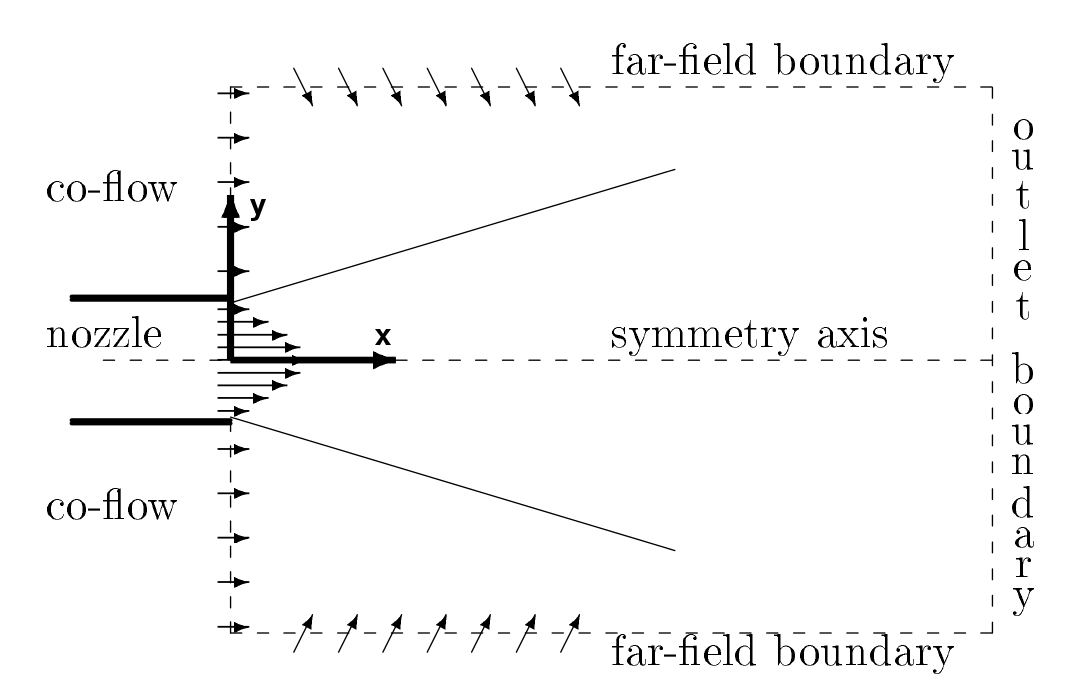
\includegraphics[width=0.75\textwidth]{./figuras/chap2/jet.png}
\end{center}
\caption{Definition of axis orientation and domain boundaries for the emerging round jet flow. Adapted from \cite{luppes}.}
\label{fig: jet_bc}
\end{figure}

Numerical solution of the equations will be performed time accurately due to the stochastic modeling of liquid atomization, as explained later in the dispersed phase section of this chapter. The initial conditions would then be the steady state solution of a pure gas jet. 

The time-dependence of thermodynamic pressure $p_0$ is neglected and it is assumed constantly equal to ambient pressure, or an unity value in dimensionless form,
\begin{equation}
 p_0 (t) = 1 \, .
\end{equation}


\subsubsection{Boundary Conditions of Turbulent Quantities}

Introduction of two new variables in the turbulence model, namely $k$ and $\epsilon$, requires the definition of their boundary conditions.

\begin{description}
 \item[Nozzle inlet conditions:]
\begin{subequations}
 \begin{align}
  k(\partial \Omega_{nozzle},t) &= k_{nozzle}(\bv{x}) \, ,\\
  \epsilon(\partial \Omega_{nozzle},t) &= \epsilon_{nozzle}(\bv{x}) \, ,
 \end{align}
\end{subequations}

\item[Co-flow conditions:]
\begin{subequations}
 \begin{align}
  k(\partial \Omega_{\text{co-flow}},t) &= k_{\text{co-flow}} \, , \\
  \epsilon(\partial \Omega_{\text{co-flow}},t) &= \epsilon_{\text{co-flow}} \, ,
 \end{align}
\end{subequations}

\item[Far-field boundaries:]
\begin{subequations}
 \begin{align}
  \frac{\partial k}{\partial \bv{n}} (\partial \Omega_b,t) &= 0 \, , \\
  \frac{\partial \epsilon}{\partial \bv{n}} (\partial \Omega_b,t) &= 0 \, ,
 \end{align}
\end{subequations}

\item[Outlet conditions:]
\begin{subequations}
 \begin{align}
  \frac{\partial k}{\partial \bv{n}} (\partial \Omega_{outlet},t) &= 0 \, , \\
  \frac{\partial \epsilon}{\partial \bv{n}} (\partial \Omega_{outlet},t) &= 0 \, .
 \end{align}
\end{subequations}
\end{description}

Functions $k_{nozzle}(\bv{x})$ and $\epsilon_{nozzle}(\bv{x})$ and scalars $k_{\text{co-flow}}$ and $\epsilon_{\text{co-flow}}$ are also determined in Chapter \ref{chap: exp}.

\section{Dispersed (Liquid) Phase}

The modeling presented for the liquid phase here is solely intended to deal with
the situation of a narrow liquid jet emerging from a nozzle in a coaxial gaseous
flow in 
specific conditions that cause the liquid jet to atomize, that is, to
disintegrate into a large number of non-contiguous small volumes called
droplets. 
Despite that, this situation is further simplified to produce results for
engineering problems and many of the physical complexities are not addressed.

The ensemble of droplets originated from atomization is called the spray.
The spray evolution in time is a complex phenomenon as the liquid droplets exchange heat, mass
and momentum with the surrounding gas and other droplets. The droplets
also have their inner thermodynamics and might become unstable to the
point where they subdivide into smaller ones.

Here, the droplets will be treated as particles with the following properties:
\begin{itemize}
 \item liquid substance: according to which the constitutive properties will be
defined (only single-component liquids are concerned, see
\cite{baumgarten2006mixture});
 \item geometric properties: all droplets are assumed to be spheric with 
diameter $D$;
 \item thermodynamic properties: pressure, volume, mass, temperature;
 \item kinematic properties: position and velocity (translational only).
\end{itemize}

This description is often called the point-particle method, see \cite{balachandar2010turbulent}.

The next subsections will describe the processes being modeled for
computation of spray evolution (the evolution of all droplet properties in time). 

The approach to the inter-phase interaction shown below is usually called the two-way coupling because it
comprises the interaction between gas and droplet but neglects the interactions between two different droplets, like
droplet collisions. It is mostly used for the case of dilute sprays, when the liquid volumetric fraction ($\phi_{v,l}$) satisfies $\phi_{v,l}<10^{-3}$.

\subsection{Atomization or Primary Break-Up}

The atomization is not modeled in a deterministic way, with the dynamics of liquid jet disintegration into droplets. 

Rather, it is used a stochastic approach called the Monte Carlo's method, see \cite{baumgarten2006mixture}, that describes resulting droplets from atomization process based on available measurements near the nozzle exit plane.

Droplets are inserted into the domain in groups called parcels. A parcel is
a group of droplets with all properties being exactly the same.
This means that one single set of ordinary differential equations is solved for
the entire group (and
not one set for each droplet) the only difference being that the parcel mass ($m_{parcel}$) is
the sum of all droplet mass ($m_d$). This means that,
\begin{equation}
 m_{parcel} = N_d m_d = N_d\left( \rho_d \frac{\pi D^3}{6}\right) \, ,
\end{equation}
where $m_d$ is the droplet mass, $N_d$ is the number of droplets represented by this parcel and $D$ is the parcel (and the droplet) diameter.


For each time instant, a certain number of parcels is inserted into the domain to represent the
liquid injection. The parcel properties in the nozzle exit are specified as either constant values or random variables sampled from statistical distributions built from experimental data.

In this work, all parcel properties in the nozzle have constant values except for the parcel diameter,
which is a random variable.


\subsection{Secondary Break-Up}

The secondary break-up of droplets is neglected. It is considered that droplets
vaporize (and either disappear or have their diameter reduced) before they
become unstable.

\subsection{Momentum Transfer}

The motion and momentum equations for a particle are:
\begin{equation}\label{eq: drop_mom}
\frac{d\bv{x}_d}{dt} =\bv{U}_d  , \quad m_d \frac{d\bv{U}_d}{dt} = \bv{F} \, .
\end{equation}

The resulting force ($\bv{F}$) on the particle  proposed by \cite{vonkarman} is here
simplified for the case of a rigid spheric droplet under small pressure
gradient and in low droplet Reynolds number. The buoyancy force is
neglected because the gas density is much lower than the liquid density ($\rho \ll \rho_d $).  The effect of mass transfer on the droplet momentum equation was also neglected so that
\begin{equation}
 \frac{d \left(m_d \bv{U}_d \right) }{dt}\approx  m_d\frac{d \bv{U}_d }{dt} \, .
\end{equation}


The droplet slip velocity (the droplet velocity relative to the gas) is given by:
\begin{equation}\label{eq: Urel}
 \bv{U}_{slip} = \bv{U_d} - \underbrace{\left( \tilde{\bv{U}}+\bv{U}'' \right)}_{\text{gas}} \, ,
\end{equation}
where $\tilde{\bv{U}}$ is the Favre-averaged gas velocity computed in Equation \eqref{av: momentum} and $\bv{U}''$ is its fluctuation.
Since $\bv{U}''$ is unknown, it is modeled as explained later in the droplet dispersion subsection.


\begin{equation}\label{eq: drop_mom_F}
 \bv{F}=-\rho\frac{\pi D^2}{8}C_D | \bv{U}_{slip}| \bv{U}_{slip}
+ m_d \bv{g} \, .
\end{equation}

where the drag coefficient and the droplet Reynolds number read:
\begin{equation}
 C_D =\begin{cases}
\frac{24}{Re_d} \left( 1 + \frac{1}{6} Re^{2/3}_d \right) & Re_d < 1000,\\
0.424 & Re_d \geq 1000.
\end{cases}
\end{equation}

\begin{equation}
 Re_d = \frac{\rho | \bv{U}_{slip}| D}{\mu} \, .
\end{equation}

Rearranging \eqref{eq: drop_mom} and \eqref{eq: drop_mom_F},
\begin{equation}\label{eq: drop_dudt}
 \frac{d\bv{U}_d}{dt} = -\frac{ \bv{U}_{slip}}{\tau_{u}} + \bv{g} \, .
\end{equation}

$\tau_u$ is the momentum relaxation time,
\begin{equation}
 \tau_u = \frac{8 m_d}{\pi \rho C_D D^2 | \bv{U}_{slip}|}=\frac{4}{3}
\frac{\rho_d D}{\rho C_D | \bv{U}_{slip}|} \, .
\end{equation}

\subsection{Heat and Mass Transfer}

In the case of an evaporating spray with the droplet temperature below the air temperature,
 energy is transfered from the gas to the droplets (heat transfer) and liquid mass is evaporating if the gas is not saturated with vapor (mass transfer). The liquid temperature will either increase or decrease depending on the rate at which each process takes place.

The droplet heating and vaporization is given a simplified treatment presented in \cite{sirignano} as infinity-liquid-conductivity model, it considers spheric symmetry for the droplet and the surrounding gas with a time varying but spatially uniform temperature of liquid phase. 

The droplet energy equation is written as
\begin{equation}\label{eq: drop_energy}
 m_d \frac{dh_d}{dt} = \frac{d m_d}{dt} L_v \left(T_d\right)+Q_d \, ,
\end{equation}
where $L_v\left( T_d\right)$ is the latent heat of evaporation at temperature $T_d$.

The modeling of heat ($Q_d$) and mass ($dm_d/dt$) tranfers  will be divided in two subsections. The heat transfer is discussed first and the mass transfer comes next.

\subsubsection{Gas-Droplet Heat Transfer}

The gas-droplet heat transfer model is developed from two basic assumptions:
\begin{itemize}
 \item Thermal diffusivity is larger in gas than in liquid: this means that changes in temperature of liquid surface instantaneously affect the surrounding gas phase, what is generally true for liquids far from critical conditions. Mathematically, this means that temperature derivatives with respect to time are neglected in the gas phase.
 \item The time required for heat diffusion from droplet surface to its interior is much smaller than the droplet lifetime (the time required for complete evaporation). 
\end{itemize}

Consider the heat flux scheme proposed in \cite{naca} and outlined in Figure \ref{fig: drop_heat}: heat is transfered from air to a film composed of air and vapor and then to the droplet. 

The droplet has a temperature $T_d$ and is surrounded by the air-vapor film whose temperature $T_f$ varies radially until it reaches the air temperature $T$ at radius $r=D/2+\delta_f$. The following heat fluxes occur:
\begin{itemize}
  \item Total heat transfered from the air to the film and the droplet: $Q$;
  \item Heat that actually arrives at droplet surface: $Q_d$;
  \item Sensible heat that increases liquid temperature: $Q_L$;
  \item Latent heat of evaporation: $L_v$;
  \item Heat transferred from air to film: $Q_S$.
\end{itemize}

And they are related by the following equation:
\begin{equation}
\begin{split}
  Q_d = Q_L + L_v & = Q - Q_S \, .
\end{split}  
\end{equation}

The enthalpy equation for the air-vapor film surrounding the droplet in spherical coordinates is:
\begin{equation}\label{eq: Qd}
 \frac{d}{dr}\left[ 4\pi r^2 h_c \frac{dT_f}{dr} - \dot{m}_d c_{p,f} \left(T_f -T_d\right)\right] =0 \, ,
\end{equation}
where $r$ is the distance from the droplet center, $h_c$ is the coefficient of convective heat transfer through the film, $\dot{m}_d$ is the rate at which vapor mass evaporates and diffuses out and $c_{p,f}$ is the specific heat in the film. They are all assumed to be constant throughout the film.

Applying the boundary condition at the droplet surface, Equation \eqref{eq: Qd} becomes:
\begin{equation}\label{eq: Qdbc}
 Q_d = 4\pi r^2 h_c \frac{dT_f}{dr} - \dot{m}_d c_{p,f} \left(T_f -T_d\right)
\end{equation}

Assuming that the film thickness is small so that:
\begin{equation}
4\pi r^2 \approx \pi D^2 \quad \text{for} \quad r \in [D/2, D/2+\delta_f] \, ,
\end{equation}
and integrating Equation \eqref{eq: Qdbc}:
\begin{equation}
\int_{D/2}^{D/2+\delta_f} dr = \int_{T_d}^{T} \frac{\pi D^2 h_c}{Q_d +\dot{m}_d c_{p,f} \left(T_f-T_d\right)}dT_f \, ,
\end{equation}
the result is the rate of heat transfer from the air to the droplet:
\begin{equation}\label{eq: Qd_final}
Q_d = \pi D^2 h_c \left( T - T_d \right)\frac{z}{e^z-1} \, ,
\end{equation}
%h_c = [W/m/K]
where
\begin{equation*}
z= - \frac{c_{p,f} \dot{m}_d \delta_f}{ \pi D^2 h_c} \, .
\end{equation*}

The expression for modeling the heat transfer coefficient - $h_c$ - is the one used by \cite{nordin},
\begin{equation}
  \frac{\pi D^2 h_c}{\delta_f} = \pi D \kappa_f Nu_f \, .
\end{equation}

Equation \eqref{eq: Qd_final} is thus: 
\begin{equation}
Q_d = \pi D \kappa Nu \left( T-T_d \right)  \frac{z}{e^z-1} \, .
\end{equation}

The Nusselt number - $Nu$ - is given by the correlation bellow and the Prandtl number - $Pr$ - is computed directly from its definition:
\begin{equation}
 Nu= 2.0 +0.6 Re^{1/2} Pr^{1/3} \, , \quad Pr = \frac{\mu_f c_{p,f}}{\kappa_f} \, .
\end{equation}

All gas properties ($c_{p,f}$, $\mu_f$ and $\kappa_f$) in the above equation should be computed using the characteristic film temperature ($T^{*}_f$) defined by the the so called one-third rule:
\begin{equation}
 T^{*}_f = \frac{2T_d + T}{3} \, .
\end{equation}

The equation for droplet energy \eqref{eq: drop_energy} may also be written in terms of temperature and characteristic time scales for heating - $\tau_h$ - and evaporation - $\tau_e$:
\begin{equation}
 \frac{dT_d}{dt}= \frac{T-T_d}{\tau_h} f - \frac{1}{c_{p,d}} \frac{L_v\left( T_d\right) }{\tau_e} \, ,
\end{equation}
where
\begin{equation}
 \tau_h=\frac{m_d c_{l,d}}{\pi D \kappa Nu} \, , \quad f =  \frac{z}{e^z-1} \, .
\end{equation}

An expression for $\tau_e$ is given by Equation \eqref{eq: tau_e}, derived in the next subsection.

\begin{figure}
 \centering
 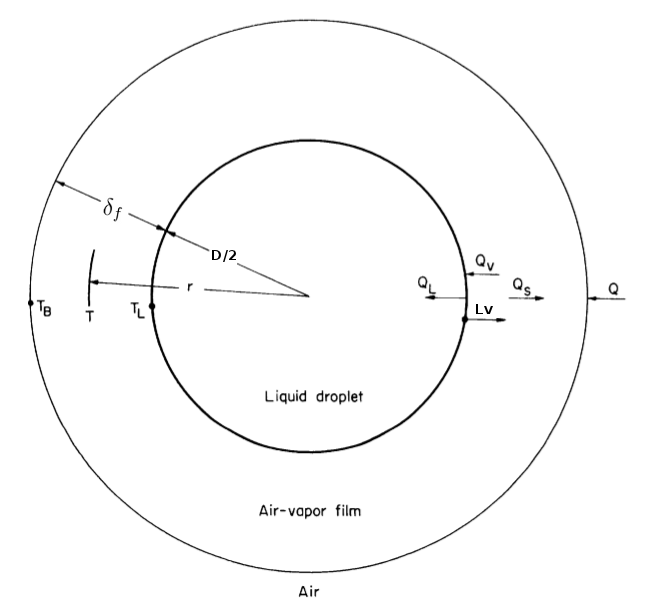
\includegraphics[width=0.8\textwidth]{./figuras/chap2/droplet_heat.png} 
 \caption{Scheme of heat flux from air to droplet, adapted from \cite{naca}.}
 \label{fig: drop_heat}
\end{figure}


\subsubsection{Mass Transfer}

The exposition below follows the already commented simplifications and is commonly denoted as $D^2$-law, see \cite{sirignano}.
Only mass transfer from the droplet to the gas is considered, thus condensation is not allowed.

The steady-state continuity equation for the surrounding gas around the droplet in spherical coordinates is:
\begin{equation}\label{eq: film_mass}
 \frac{d}{d r} \left( \rho u r^2 \right) = 0 \quad \rightarrow \quad \rho u r^2 = cte \, ,
\end{equation}
where $r$ is the radial coordinate and $u$ is the radial velocity.

Using the boundary condition at droplet surface,
\begin{equation}\label{eq: film_species_bc}
 \dot{m}_d = \rho u \left( 4\pi r^2  \right) \, .
\end{equation}
 

The steady-state species equation is:
\begin{equation}\label{eq: film_species}
\frac{d}{d r} \left[ 4\pi r^2 \left( \rho u Y_v -\rho \mathcal{D}_v  \frac{d Y_v}{d r}  \right)\right] = 0\, ,
\end{equation}
where $Y_v$ is the vapor mass fraction and $\mathcal{D}_v$ is the vapor diffusion coefficient. The boundary condition at droplet surface is:
\begin{equation}\label{eq: film_species_bc}
 \left\lbrace 4\pi r^2 \left[ \rho u Y_v -\rho \mathcal{D}_v  \frac{d Y_v}{d r} \right]\right\rbrace  _{r=D/2}  = \dot{m}_d\, . \\
\end{equation}

The integral of \eqref{eq: film_species} using \eqref{eq: film_mass} and \eqref{eq: film_species_bc} may be written as:
\begin{equation}
-\int_{D/2}^{\infty} \frac{\dot{m}_d}{4\pi \rho \mathcal{D}_v}\frac{dr}{r^2} = \int_{Y_{v,s}}^{Y_{v,\infty}} \frac{dY_v}{1-Y_v} \, ,
%- \rho D_v \frac{d Y_v}{d r} = \frac{\dot{m}_d}{4\pi r^2}\left(1-Y_v\right) \, .
\end{equation}
where $Y_{v}$ is the vapor concentration in the air-vapor film. Performing the integration, it becomes:
\begin{equation}
 \frac{dm_d}{dt} = -2\pi D \mathcal{D}_v \rho_v ln \left(
\frac{1-Y_{v,\infty}}{1-Y_{v,s}} \right) \, .
\end{equation}


The vapor mass fraction near the droplet surface ($Y_{v,s}$) is obtained assuming liquid-vapor equilibrium. In this situation, the vapor partial pressure ($p_v$) is given by Clausius-Clapeyron equation:
\begin{equation}
ln \left(\frac{p_v}{p_\infty}\right) = -\frac{L_v W_{v}}{R} \left(\frac{1}{T_d}-\frac{1}{T_b}\right) \, ,
\end{equation}
where $T_b$ is the liquid boiling temperature at pressure $p_{\infty}$ and $L_v$ is the heat of vaporization per unit mass.

Using Raoult's law and the ideal gas state equation, the vapor mass concetration near droplet surface ($Y_{v,s}$) is:
\begin{equation}
Y_{v,s} = \frac{p_v \left(T_d\right)}{p}\frac{W_v}{W} \, .
\end{equation}


The extra mass transfer due to gas motion around the droplet is accounted by the Sherwood number given by the empirical correlation of \cite{ranzmarshall}:
\begin{equation}\label{eq: dropxxxmass}
 \frac{dm_d}{dt} = -2\pi D \mathcal{D}_v \rho_v ln \left(
\frac{1-Y_{v,\infty}}{1-Y_{v,s}} \right) Sh \, ,
\end{equation}
where
\begin{equation}
 Sh = 2.0 +0.6 Re^{1/2} Sc^{1/3} \, .
\end{equation}
As for the Nusselt number, all properties here are computed with the characteristic film temperature ($T^{*}_f$) previously defined.

The droplet evaporation rate ($dm_d/dt$) may then be written as:
\begin{equation}
 \frac{dm_d}{dt}=-\frac{m_d}{\tau_e} \, ,
\end{equation}
where
\begin{equation}\label{eq: tau_e}
 \tau_e = \frac{m_d}{\pi D \mathcal{D} Sh \rho_v ln \left(
\frac{1-Y_{v,\infty}}{1-Y_{v,s}} \right)}
\end{equation}
is the characteristic time scale of droplet evaporation.



% 
% For a droplet temperature above the boiling point, the evaporation occurs at constant temperature and the mass transfer is determined by the rate at which energy is transfered from the gas to the liquid, sustaining the phase change. The equations bellow 
% 
% \begin{equation}
%  \frac{dm_d}{dt}=-\frac{\pi D \kappa Nu}{c_{p,v}} ln \left[ \frac{c_{p,v}}{L_v}
% \left( T- T_d \right) +1 \right]
% \end{equation}
% 
% 
% \begin{equation}
%  \frac{dD}{dt} = -\frac{D}{\tau_{boil}}
% \end{equation}
% 
% \begin{equation}
%  \tau_{boil} = \frac{D^2 \rho_d c_{p,v}}{2 \kappa Nu ln \left[
% \frac{c_{p,v}}{L_v} \left( T- T_d \right) +1 \right]}
% \end{equation}

\subsection{Droplets at Domain Boundaries}

When the droplet crosses the domain boundary, it is simply removed from the computation.

\subsection{Droplet Dispersion}

Although the gas phase velocity has been averaged in \eqref{av: momentum}, the droplet experiences oscillations in its slip velocity if turbulence is present.
This oscillation not only affects the droplet drag, the extra shear on droplet surface might cause deformation and instabilities leading to droplet break-up.
Furthermore, due to changes in the surrounding gas flow, mass and heat transfers are also affected. 

Here, the effects of turbulence on droplet motion are simply accounted for by summing a fluctuation ($\bv{U}''$) to the gas averaged velocity ($\tilde{\bv{U}}$):
\begin{equation}
  \bv{U}_{slip} = \bv{U_d} - \left( \tilde{\bv{U}}+\bv{U}'' \right) \, . \tag{\ref{eq: Urel}}
\end{equation}

For the k-epsilon model, a characteristic magnitude for velocity fluctuation may be defined as the scalar
\begin{equation}
 <U''>= \sqrt{\frac{2}{3} k} \, .
\end{equation}

The magnitude of the velocity fluctuation ($\bv{U}''$) is then sampled from a Gaussian distribution with a variance equal to $<U''>$ and zero mean. Finally, the direction of $\bv{U}''$  is randomly chosen.

The sampling is performed once the time passed from the last sampling is greater than the characteristic time $\tau_{turb}$: the minimum between the eddy lifetime and the time taken to the droplet to cross it, given by the ratio of a turbulent length scale ($l_t = C_{\mu}^{3/4} k^{3/2} / \epsilon $) and the magnitude of the droplet slip velocity:

\begin{equation}
 \tau_{turb} = min \left[ \frac{k}{\epsilon} , \frac{k^{3/2}}{\epsilon} \frac{C_{\mu}^{3/4}}{|\bv{U}_{slip}|}\right] \, .
\end{equation}

Further details are discussed in \cite{kiva} and \cite{baumgarten2006mixture}.
